\section{Detailed Circuit Description}
\subsection{Power Input Circuit}

This instrument is complex and has many somewhat expensive parts, so a full
input subsystem was designed to ensure that these parts are always supplied
correctly with power. This subsystem provides the following features:

\begin{itemize}
\item{Overcurrent protection}
\item{Reverse polarity protection}
\item{Undervoltage lockout}
\item{Overvoltage protection}
\item{Inrush current limiting}
\end{itemize}

\subsubsection{Overcurrent protection}

The first piece of this input system, and possibly the simplest, is
\refdes{R81}. \refdes{R81} is a \emph{resettable fuse}, a type of resistor
with a positive temperature coefficient. Its resistance is very low
(around $0.5\;\Omega$) at room temperature.  As the current flowing through it
increases, it heats up, and as it heats up, its resistance increases.
Eventually, it will reach a point where this process `snowballs', and its
resistance is high enough that almost no current can flow through it. This
allows it to act like a fuse, but without permanently blowing: as soon as it
cools back down, it will conduct again.

\begin{figure}[H]
\centering
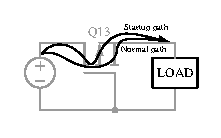
\includegraphics[width=3in]{mosrpp}
\caption{MOS reverse polarity protection circuit, simplified}
\label{fig:mosrpp}
\end{figure}

\subsubsection{Reverse polarity protection}

Once input current has passed through the resettable fuse, it encounters
\refdes{Q13}. A simplified form of this part of the circuit can be seen in
figure~\ref{fig:mosrpp}. Remember that a MOSFET has `parasitic' diodes
connected from the transistor's channel to its substrate; in a
standard power MOSFET, one ends up connected between the two ends of the
channel (the other ends up shorted to itself). In a P-channel MOSFET, this
diode points from the source to the drain. In this circuit, when power is
applied with the correct polarity, this diode allows current to initially take
the path labeled \emph{startup path}. When it does so, the voltage applied to
the load begins to rise, but the gate stays low, as it is tied to ground.
Eventually, the voltage rises high enough that the gate-source voltage switches
on the MOSFET, and current begins to flow through the \emph{normal path}
instead. This path takes the current through the low-impedance MOSFET channel,
rather than through the diode where the forward threshold voltage of the diode
would be lost.

If power is applied in the incorrect polarity, the substrate diode never
conducts, so the MOSFET never switches on.

\subsubsection{Power switch}

After the reverse polarity protection, the current must flow through
\refdes{Q14}, which is connected as a traditional switch. \refdes{R88} holds
its gate and source together when the power is switched off, keeping the MOSFET
also turned off.

%\end{multicols}
\begin{figure}[H]
\centering
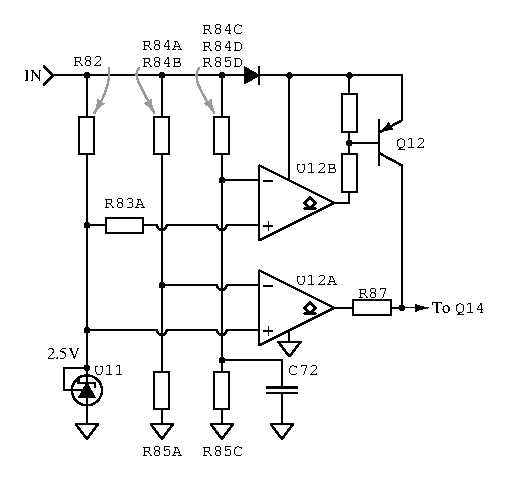
\includegraphics[width=3in]{comparator}
\caption{UVLO and OVLO circuit}
\label{fig:uovlo}
\end{figure}
%\begin{multicols}{2}

To simplify things, the subcircuit in figure~\ref{fig:uovlo} is powered through
a single diode for its own reverse-polarity protection. Bandgap voltage reference
\refdes{U11} does not need this, as its internal circuit has an antiparallel diode
built in~\cite{tl431}.

\subsubsection{Undervoltage lockout}

\refdes{U11} provides an accurate $2.5\;\mr{V}$ level against which the input
voltage can be compared. As the input voltage rises, the voltage at the output of
the \refdes{R84A}/\refdes{R84B}/\refdes{R85A} voltage divider also rises. When
this divided voltage reaches the $2.5\;\mr{V}$ reference level, the input voltage
is at $7.5\;\mr{V}$, the undervoltage threshold. Comparator \refdes{U12A}
switches low, allowing power switch \refdes{Q14} to switch on and allow the
full system to operate.

\subsubsection{Overvoltage protection}

If the input voltage continues to rise, the voltage at the output of the
\refdes{R84C}/\refdes{R84D}/\refdes{R85D}/\refdes{R85C} voltage divider will
eventually reach the reference level when the input voltage is at $10\;\mr{V}$.
\refdes{C72} provides a low-pass effect which prevents simple noise and short
transients from causing this. When this happens, comparator \refdes{U12B}
switches low. At this point, two things happen. First, \refdes{Q12} switches
\refdes{Q14} off, powering down the circuit. Second, \refdes{D5} pulls the
reference level as seen by \refdes{U12B} down to about $1\;\mr{V}$, locking
the system in this shutdown mode until the input voltage drops back as low
as $4\;\mr{V}$ --- at which point it must climb again to the $7.5\;\mr{V}$
undervoltage threshold. In practice, the system must be powered off and back
on. This latch prevents the instrument from accidentally being powered by
too high an input voltage.

\subsubsection{Inrush current limiting}

\refdes{Q14} does not act \emph{only} as a power switch. When it switches on,
it starts in the `cutoff' region of operation, and moves to the `saturation'
region. However, it must pass through the `linear' region. We can take
advantage of this.

\begin{figure}[H]
\centering
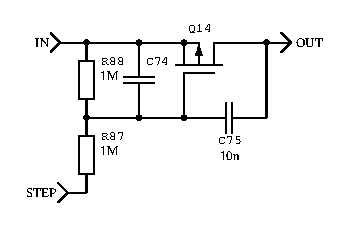
\includegraphics[width=3in]{millerint}
\caption{Miller integrator}
\label{fig:miller}
\end{figure}

The circuit in figure~\ref{fig:miller}, when \refdes{Q14} is in the linear
region, is known as a `Miller integrator'~\cite[pg. 283]{tranckts-sawtooth}.
Because \texttt{R87} and \texttt{R88} form a voltage divider, the input
voltage to the integrator will be half the input supply voltage at half
the resistance (nominally, $4.5\;\mr{V}$ at $500\;\mr{k\Omega}$). The
integrator capacitance is simply \texttt{C75}, which is $10\;\mr{nF}$.
Because the voltage across \texttt{C74} changes only negligibly, its effect
on the circuit will also be negligible.

At startup, \refdes{C75} would tend to hold the gate above the source,
switching the transistor fully on and bypassing any limiting effect. The
much larger \refdes{C74} swamps this effect, holding the gate to the
source until a DC source of current is provided via \refdes{R87}.

The input signal to this integrator will be a step, because comparator
\texttt{U12A} switches directly from `off' to `on'. Integrating a step gives
a ramp, with a slope of:

\begin{equation*}
    \frac{dv}{dt} = \frac{v_\mr{in}}{RC} = \frac{4.5\;\mr{V}}{(500\;\mr{k\Omega})(10\;\mr{nF})}
    = 900\;\mr{V/s} = 0.9\;\mr{V/ms}
\end{equation*}

This means it will take about $10\;\mr{ms}$ for the voltage to ramp from zero
to the full input voltage of $9\;\mr{V}$.

Because the inrush current to be limited is the current charging the system's
capacitance, we can calculate the worst-case inrush current. Charge is held
on-board by approximately $200\;\mr{\mu F}$ worth of capacitors. Given this
capacitance and the voltage slope, the current is calculated as follows:

\begin{equation*}
    I = C \frac{dv}{dt} = (200\;\mr{\mu F})(900\;\mr{V/s}) = 180\;\mr{mA}
\end{equation*}

During this charging time, the power dissipated in \texttt{Q14} will be high.
The worst-case is when the full input voltage is dropped across it, giving
a power dissipation of $(9\;\mr{V})(180\;\mr{mA}) = 1.62\;\mr{W}$. The average
power for the entire time will be:

\begin{gather*}
    P = IV \\
    P_\mr{avg} = \frac{1}{10\;\mr{ms}}\int_0^{10ms} iv\;dt \\
    {}= \tfrac{1}{2}(1.62\;\mr{W})(10\;\mr{ms})/(10\;\mr{ms}) \\
    {}= 810\;\mr{mW} \\
\end{gather*}

Thus, a MOSFET must be selected that can handle an $810\;\mr{mW}$ pulse for
$10\;\mr{ms}$. This pulse-handling capability is shown in the datasheet as
the ``forward-biased safe operating area'', and we selected an AOD417 which
can easily handle this pulse with excess~\cite{aod417}.

\begin{figure}[H]
\centering
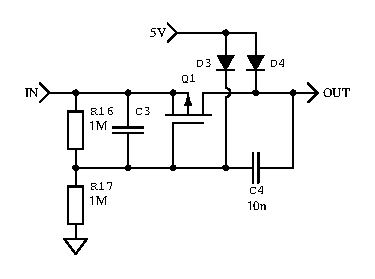
\includegraphics[width=3in]{usbinput}
\caption{USB power input circuit}
\label{fig:usbpower}
\end{figure}

\subsubsection{USB Power Input Circuit}

The USB specification is very demanding with respect to the amount of inrush
current that a USB device may consume. We used the same Miller-integrator
inrush limiting circuit on the USB power supply input.

In this case, the resistance has not changed (still a Th\'evenin-equivalent
$500\;\mr{k\Omega}$), and the input step is equal to $2.5\;\mr{V}$, half the
input voltage. The integrating capacitance is \refdes{C4}, which has a value of $10\;\mr{nF}$,
and the maximum input capacitance being charged is approximately $20\;\mr{\mu F}$.

\begin{gather*}
    \frac{dv}{dt} = \frac{v_\mr{in}}{RC} = \frac{2.5\;\mr{V}}{(500\;\mr{k\Omega})(10\;\mr{nF})}
    = 500\;\mr{V/s} \\
    I = C \frac{dv}{dt} = (20\;\mr{\mu F})(500\;\mr{V/s}) = 10\;\mr{mA}
\end{gather*}

The power dissipation in this case is very small (no more than $50\;\mr{mW}$ for
only a few milliseconds), so we used a smaller and less expensive MOSFET that
was already in use elsewhere for this particular integrator.

No reverse polarity protection was deemed necessary on the USB input.

Diodes \refdes{D3} and \refdes{D4} allow the on-board power supply to power
the circuitry downstream from the USB port whenever that supply is powered,
so that this circuitry can draw larger amounts of current without the trouble
of making sure that this current draw is within USB specifications.
\refdes{D3} shuts off \refdes{Q1}, and \refdes{D4} provides power in
\refdes{Q1}'s absence.


\subsection{Switching DC-DC Converters}

\begin{figure}[H]
\centering
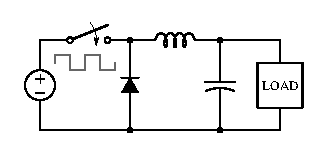
\includegraphics[width=3in]{buckconv}
\caption{Basic buck converter circuit}
\label{fig:basicbuck}
\end{figure}

\subsubsection{Buck converter theory}

The basic idea of an inductor is that it translates electric current flowing
through it into a magnetic field around it. There is energy stored in this
magnetic field, so the inductor tends to hold the current fixed (as changing
the current would require adding or removing energy from the field). The
`buck converter' is a voltage down-converter circuit that takes advantage
of this.

A more mathematical approach is that inductors integrate the voltage applied
to them, producing a current:

\begin{equation*}
    i = \frac{1}{L} \int v\;dt
\end{equation*}

A buck converter must have at least one switch, as shown in
figure~\ref{fig:basicbuck}.  The switch is initially closed for a brief period.
This applies a positive voltage to the inductor, causing the current through it
to begin to increase (remember that the integral of a step is a ramp). This
current flows through to the output of the converter, and the output voltage
begins to rise.

Now, the switch is opened. The inductor keeps the current flowing, though,
through the diode this time. The voltage across the inductor is now negative
(the voltage on the left side had to fall negative in order to forward-bias the
diode and make it conduct), so the current starts ramping downward, and the
output voltage begins to fall.~\cite[pp.~356--357]{aoe-vreg}

By repeating this cycle, the output voltage can be made to rise and fall around
a desired point, and by placing a large capacitor at the output, the rising and
falling current can translate to very small variation in output voltage, though
it must rise and fall at least a small amount. This allows the output voltage
to be any arbitrary voltage smaller than the input voltage, but does not
theoretically lose power, unlike a linear regulator (whose entire mechanism of
operation is intentional power loss).


\begin{figure}[H]
\centering
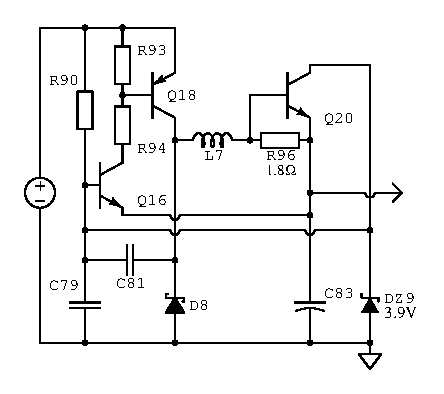
\includegraphics[width=3in]{3v3buck}
\caption{$3.3\;\mr{V}$ buck converter circuit}
\label{fig:3v3buck}
\end{figure}

\subsubsection{3.3 V buck converter}

In this instrument, we have used a simple, three-transistor regulated buck
converter circuit. It is inexpensive, reliable, and though it is not hugely
efficient, it generates relatively little switching noise (due, in part, to
its low speed compared to more modern designs).

In the first phase of the switching cycle, \refdes{Q16}'s base voltage is
low. \refdes{R90} charges \refdes{C79}, and eventually the base voltage rises
high enough that \refdes{Q16} switches on. It pulls \refdes{Q18}'s base voltage
down, switching on that transistor too. \refdes{Q18} is equivalent to the main
switch in figure~\ref{fig:basicbuck}, and the inductor current starts to rise.

In the next phase of the switching cycle, something draws current towards ground
out of \refdes{C79} and away from \refdes{Q16}'s base. This starts a chain reaction:
\refdes{Q16} and \refdes{Q18} start to switch off, and are no longer driving the
inductor. The inductor's tendency to keep current flowing makes the voltage on its
left side sharply decrease. This decrease is coupled through \refdes{C81}, which
drags \refdes{Q16}'s base voltage even lower, switching it off quite solidly.
The converter will remain switched off until \refdes{C79} charges back up through
its resistor.

Two things can be the `something' of the previous paragraph, initiating the
switch from phase 1 to phase 2. First, note that \refdes{Q16}'s emitter is
connected to the output voltage, so when it is switched on, its base will be
about $0.65\;\mr{V}$ above that. When the output voltage reaches about
$3.25\;\mr{V}$, the base voltage is at about $3.9\;\mr{V}$, and Zener diode
\refdes{DZ9} starts to conduct. This means that the output voltage will not be
allowed to rise above about $3.25\;\mr{V}$, providing the voltage regulation
function.

The inductor current must also flow through sense resistor \refdes{R96}. If the
current exceeds about $650\;\mr{mA}$, the base-emitter voltage applied to
\refdes{Q20} will be high enough to switch it on, and \refdes{Q20} will draw the
shutdown current. This provides the current-limiting function.

\subsubsection{-9V inverting regulator}
It is possible to repurpose a buck converter circuit as an inverting
(buck-boost) circuit that generates a negative voltage~\cite{buckinv}. The
circuit is otherwise the same, with two exceptions. First, the Zener diode, now
\refdes{DZ10}, is a $10\;\mr{V}$ part, giving a regulated output voltage of
about $9.35\;\mr{V}$. Second, because the current through the output capacitor
has more hard edges in a buck-boost converter, a $1\;\mr{\mu F}$ ceramic
capacitor (useful to higher frequencies and currents) has been added in
parallel with the main output capacitor.

\subsection{Linear Regulators}
A series-type linear regulator works by acting as a controlled resistance,
regulating itself to exactly the resistance required to give the correct
output voltage considering the amount of current flowing through it. This
means that power loss is a required property of linear regulators. For example,
a linear regulator taking an input voltage of $9\;\mr{V}$, giving an output
voltage of $5\;\mr{V}$, and passing a current of $100\;\mr{mA}$, will
lose $(9-5)(0.1)\;\mr{W} = 400\;\mr{mW}$ of power, dissipated as heat.
The loss is sometimes a fair trade for simplicity and low output noise.
This instrument uses four linear regulators, which provide power supplies
of $5\;\mr{V}$, $-5\;\mr{V}$, $1.8\;\mr{V}$, and a low-power $3.3\;\mr{V}$
supply (a high-power $3.3\;\mr{V}$ supply for the synthesizer comes from
the buck converter).

These regulators are \refdes{U13}, \refdes{U14}, \refdes{U15}, and \refdes{U16}.
They are monolithic devices with no external circuitry except for filter
capacitors, and as such will not be addressed further. See their datasheets for
more information:~\cite{l78m05}~\cite{mc79m00}~\cite{az1117c}~\cite{mcp1700}.

\subsection{Microcontroller}
\subsubsection{USB Communications}

\subsection{Synthesizer}

\subsection{Synthesizer Output Amplifiers}

\subsection{Output System}

\subsubsection{Attenuator and Filter}
\subsubsection{Gain Stages and Termination}

\subsection{Input System}

\subsubsection{Protection}
\subsubsection{Switching}
\subsubsection{Buffer and Filter}
\subsubsection{Logarithmic Detector}
